\section{Extreme Programming Explained}
% 2 XP's: 2000 and 200? - differences.
% General introduction to XP2k
Extreme Programming is supposed to be a lightweight, efficient, and fun approach to developing software.
One of its core points, and one of the reasons we chose XP, is the fact it contains development oriented practises.

\noindent XP is based on the four values \textit{Communication, Courage, Feedback, and Simplicity}, which are implemented through the use of the 12 practises:

\begin{tabularx}{\textwidth}{X X X}
	40-hour Week				 & Coding Standards & Collective Ownership \\
	Continuous Integration	  & Metaphor         	 & On-site Customer     \\
	Pair Programming			& Planning Game		& Refactoring          \\
	Simple Design          		  & Small Releases   	& Testing             
\end{tabularx}

These practises support each other (e.g. a coding standard supports pair programming), in such a way it creates a synergistic effect.
The complete map of which practises support each other, can be seen in \Cref{fig:practiceSupport}.
\begin{figure}[H]
	\centering
	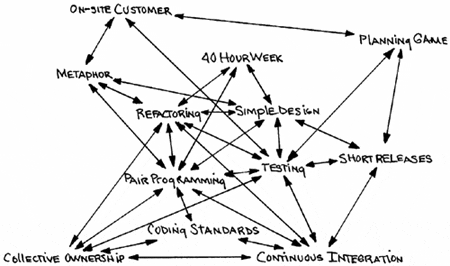
\includegraphics[scale=0.85]{Images/xpPracticeSupport.png}
		\caption{Map of the practises and how they support each other.
			From \textit{Extreme Programming Explained (1999)} \citep[p. 70]{xp:explained}. }
	\label{fig:practiceSupport}
\end{figure}

\paragraph{40-hour Week} is the suggested length of a work week in an XP project.
The relatively short week is practised because one needs to be on the top of their game when working.
Being well rested and energised should reduce the number of mistakes, as well as increase patience when pair programming.

\paragraph{Coding Standards} reduce the time it takes to understand code written by others.
A coding standard also ensures that all developers write code the same way.
This facilitates refactoring, pair programming, and encourages collective ownership.

\paragraph{Collective Ownership} allows everyone to refactor and review the code.
When no one person owns part of the code, collaboration is enforced while tedious change requests are avoided.

\paragraph{Continuous Integration} is used to build the program several times a day.
This keeps everybody up to date with the latest code changes, avoiding development on fragmented versions.

\paragraph{Metaphor} is used as a shared vision for the project.
The metaphor is used to standardise the names of variables, methods, and classes. 
This standardisation should help team members to intuitively understand the purpose of the variable, method, or class.

\paragraph{On-site Customer} is an integral role in an XP project.
The on-site customer is responsible for making decisions about priorities, requirements, and answering questions.

\paragraph{Pair Programming} is the way to code in an XP project.
It is when two developers work together on the same computer.
While one writes the code, the other analyses and comes with suggestions for improvement.
Development should be seen as a dialogue between the two developers.

\paragraph{Planning Game} is the event where the customer writes user stories, after which the developers estimate them according to cost.

\paragraph{Refactoring} is the practise used to improve the quality of the internal code without changing the external behaviour. Refactoring should also improve readability, and thereby maintainability.

\paragraph{Simple Design} is when every piece of code justifies its own existence. The code should not have any duplicated logic, and have the fewest possible classes and method. %A simple design is the best design. For the practise to work, the code must pass all unit- and acceptance tests. Further, the best design should not  code.

\paragraph{Small Releases} are small and frequent versions of the software, which are tested by the customer.
These releases incrementally complete the system.

\paragraph{Testing} refers to how the stories and releases are not complete, before they pass their respective tests. It is a mindset in which, unit tests are developed before the code (Test-Driven Development).

%http://www.techrepublic.com/article/extreme-programming-do-these-12-practices-make-perfect/
